\chapter{Deskripsi Solusi}
\label{chapter-3}

Bab ini membahas deskripsi umum permasalahan \textit{capstone}, analisis masalah
simulasi yang sudah ada, analisis terhadap objek dan lingkungan yang akan
diimplementasi, analisis solusi yang akan diterapkan untuk mengatasi masalah.

\section{Deskripsi Umum Permasalahan \textit{Capstone}}

Proyek trem otonom menggunakan simulasi untuk mempercepat dan mempermudah
pengujian dan validasi pengembangan model/algoritma \textit{decision making},
persepsi, \textit{localization}, dan \textit{mapping} trem otonom. Tim
\textit{capstone} Tugas Akhir ini merupakan bagian dari tim simulasi yang
bertugas untuk mengembangkan simulasi yang sudah ada. Kemajuan
pengembangan simulasi atau pengembangan SILS dan HILS adalah sebagai berikut:

\begin{enumerate}

	\item Eksplorasi kakas CARLA sebagai simulator.

	CARLA versi 0.9.12 diinstal. Model angkot dan becak telah diimpor
	sebagai objek statis (bukan kendaraan). Kendaraan model \textit{FireTruck}
	digunakan sebagai \textit{ego vehicle} menggantikan trem untuk sementara
	waktu karena model trem belum diintegrasi sebagai kendaraan.

	\item \textit{Web service} telah diimplementasi sebagai jalur komunikasi
	antara simulator CARLA dan Pegasus pada HILS.

	Komunikasi menggunakan \textit{web service} lambat karena jumlah transaksi
	per detik kecil dan simulasi juga lambat. Eksplorasi CARLA ROS Bridge
	dilakukan namun masih belum selesai.

	\item Menguji sensor virtual, mencoba menjalankan algoritma \textit{decision
	making} dan persepsi.

	Sensor virtual diuji apakah layak untuk digunakan sebagai pengganti sensor
	asli. Algoritma \textit{decision making} dan persepsi diuji juga pada HILS.

	\item Membuat rancangan skenario simulasi.

	Rancangan daftar skenario simulasi untuk menguji berbagai skenario dengan
	variabel cuaca, waktu, kecepatan trem, dan lalu lintas yang berbeda.

\end{enumerate}

Dari kemajuan proyek dari tahun sebelumnya dibutuhkan  penyempurnaan algoritma
persepsi berbasis sensor, perbaikan arsitektur HILS atau komunikasi yang
memadai, dan integrasi objek lokal pada skenario simulasi. Tim \textit{capstone}
yang beranggotakan 3 orang bertanggung jawab untuk:

\begin{enumerate}

	\item Mengembangkan mekanisme komunikasi antarperangkat dalam arsitektur
	HILS yang lebih lancar dan lebih cepat.
	\item Membuat implementasi skenario pengujian simulasi.
	\item Mengintegrasikan dan/atau mengimplementasikan objek lokal ke skenario
	simulasi.

\end{enumerate}

Tugas Akhir ini bertujuan untuk mengimplementasikan objek trem, objek lokal
lingkungan Indonesia di simulasi menggunakan CARLA agar lingkungan simulasi
menyerupai lingkungan aslinya sehingga mendukung pengembangan pengujian dan
validasi \textit{decision making} dan persepsi dengan menggunakan simulasi.

\section{Analisis Masalah Simulasi dan Aset Simulasi}

Simulasi trem otonom untuk saat ini telah diinisiasi namun baru sebatas
eksplorasi simulator CARLA dengan menambahkan kendaraan angkot dan becak sebagai
objek statis (bukan kendaraan) dan mengetes data dari sensor di \textit{ego
vehicle} dalam simulasi. Aset model 3D sudah dibangun namun belum
diimplementasikan ke dalam simulasi. Aset model 3D tersebut adalah: trem,
angkot, becak, sepeda onthel, sepeda motor, beberapa rambu lokal, dan gerobak.
Gambar \ref{fig:3d-model-assets} menunjukkan aset model 3D yang telah dibuat.

\begin{figure}[!tb]
% \begin{figure}[ht]
	\centering
	\subfloat[Trem]{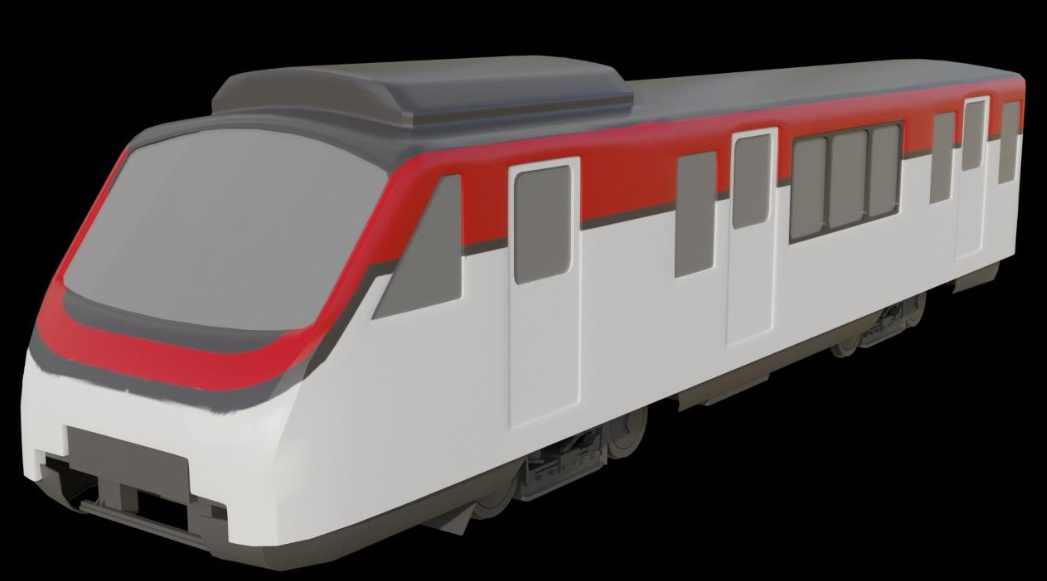
\includegraphics[width=0.4\textwidth]{resources/chapter-3-tram.png}}
	\hfill
	\subfloat[Angkot]{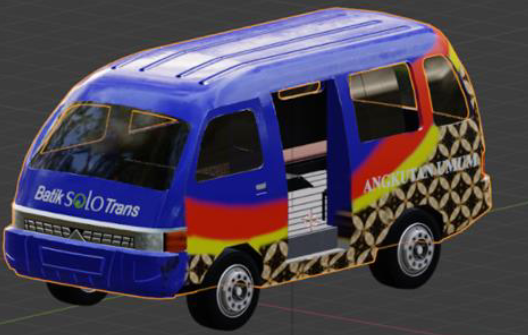
\includegraphics[width=0.4\textwidth]{resources/chapter-3-angkot.png}}
	\hfill
	\subfloat[Becak]{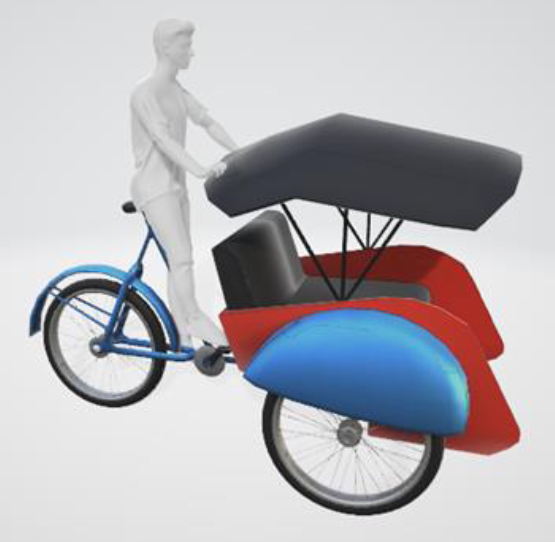
\includegraphics[width=0.3\textwidth]{resources/chapter-3-becak.png}}
	\hfill
	\subfloat[Sepeda onthel]{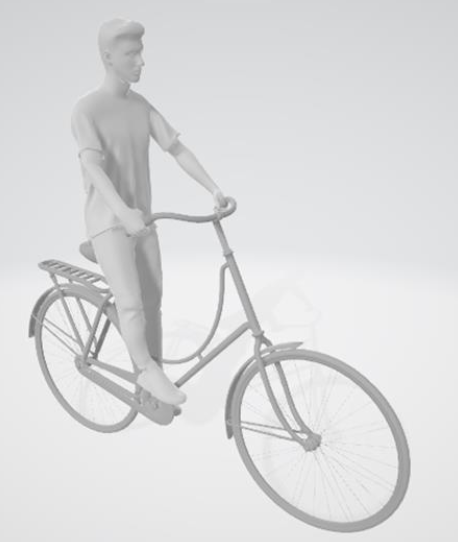
\includegraphics[width=0.3\textwidth]{resources/chapter-3-sepeda-onthel.png}}
	\hfill
	\subfloat[Sepeda motor]{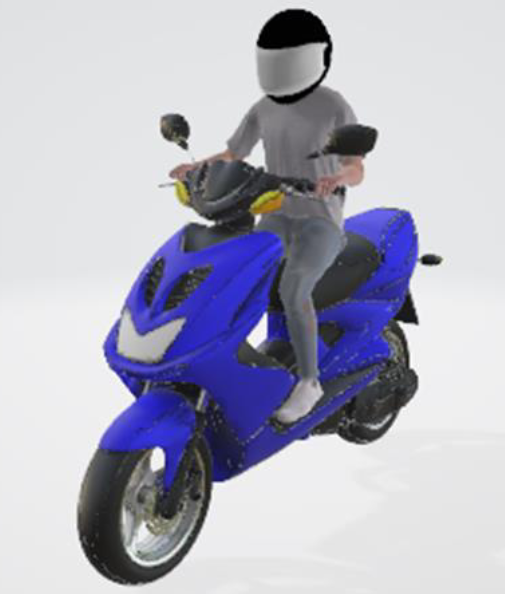
\includegraphics[width=0.3\textwidth]{resources/chapter-3-sepeda-motor.png}}
	\hfill
	\subfloat[Rambu-rambu lalu lintas]{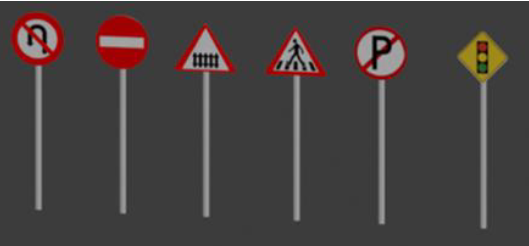
\includegraphics[width=0.4\textwidth]{resources/chapter-3-rambu.png}}
	\hfill
	\subfloat[Gerobak]{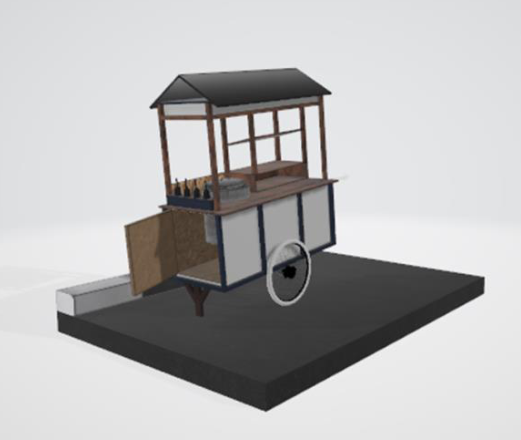
\includegraphics[width=0.4\textwidth]{resources/chapter-3-gerobak.png}}
	\caption{Aset model 3D \parencite{rispro-trilaksono}}
	\label{fig:3d-model-assets}
\end{figure}

Selain aset angkot dan becak yang diimpor sebagai objek statis, aset simulasi
untuk saat ini baru berupa aset bawaan dari CARLA. Aset bawaan CARLA seperti
peta kota, kendaraan, bangunan, rambu lalu lintas, dan lain-lain merupakan aset
yang mencerminkan kota-kota di Amerika Serikat pada umumnya. Implementasi objek
dan lingkungan Indonesia dibutuhkan agar simulasi serupa dengan kehidupan nyata
di Indonesia sehingga ketika pengujian strategi kemudi trem otonom memiliki
tingkat akurasi dan presisi yang tinggi. Simulasi yang sesuai dengan keadaan
aslinya sangat berpengaruh terhadap sistem trem otonom. Diperlukan penambahan
aset model 3D lain yang juga perlu diimplementasikan pada simulasi. Aset
tersebut adalah stasiun trem, rel trem, dan rambu yang lengkap.

Modul simulasi ini merupakan bagian dari pengembangan sistem otonom dengan
menggunakan kecerdasan buatan untuk trem. Modul ini bertujuan untuk memenuhi
kebutuhan pengujian virtual strategi kemudi trem otonom dengan simulasi.
Simulasi ini bertujuan untuk melakukan validasi strategi kemudi kecerdasan
buatan trem otonom yang telah dikembangkan. Validasi diperlukan agar kecerdasan
buatan yang dikembangkan dapat beroperasi dengan lancar di lingkungan Indonesia.
Oleh karena itu, dibutuhkan aset simulasi yang sesuai dengan keadaan Indonesia.

\section{Analisis Solusi}

Permasalahan yang telah dibahas dapat diselesaikan dengan mengubah aset yang
sudah ada dan menambahkan aset baru. Aset baru yang lain dapat dibuat
menggunakan aplikasi \textit{3D modelling}. Aset dibuat secara lengkap dan rinci
agar perilaku aset sesuai dengan yang asli.

% the sentence below goes after the first sentence
% Aset seperti peta kota harus dibuat langsung menggunakan editor CARLAUE4 atau
% menggunakan RoadRunner kemudian diimpor ke dalam editor CARLAUE4 jika aset
% peta diperlukan.

Aset model 3D yang telah jadi selanjutnya diimpor ke dalam editor CARLAUE4.
Proses impor aset ini dilakukan dengan mengikuti panduan yang telah tersedia di
dokumentasi CARLA. Proses impor aset harus dilakukan dengan benar agar perilaku
aset baik dan stabil untuk simulasi. Terdapat aset khusus yang harus ditambahkan
ke dalam berkas 3D model kendaraan dan diatur ke model kendaraan. Aset khusus
tersebut merupakan aset \textit{armature} untuk \textit{rigging} roda kendaraan.
Setelah pengaturan aset dalam editor CARLAUE4 selesai, dilakukan verifikasi aset
dengan cara menjalankan simulasi dan mengamati cara kendaraan beroperasi.
Implementasi aset berupa kendaraan bus telah berhasil dilakukan pada penelitian
lain \parencite{related-work-xiang}. Proses implementasi kendaraan bus dilakukan
dengan membuat model 3D bus, mengimpor model 3D bus ke dalam editor CARLAUE4,
mengedit aset bus tersebut dalam editor CARLAUE4, dan memverifikasi hasil impor
aset bus tersebut.

Implementasi objek dan lingkungan Indonesia yang akan dilakukan adalah dengan
menambahkan aset, membuat aset baru, dan mengubah aset yang sudah ada.
Implementasi yang menambahkan aset meliputi kendaraan, rambu lalu lintas, rel,
dan lingkungan sederhana. Kendaraan yang akan diimplementasikan adalah trem
otonom, angkot, becak, motor, dan sepeda onthel. Trem akan dipasangkan
berbagai sensor, seperti LIDAR, radar, kamera RGB untuk menangkap lingkungan
sekitar.

% note: gerobak is not going to be implemented

Pada proses implementasi aset membutuhkan simulator CARLA, CARLAUE4, dan editor
CARLAUE4 yang dibangun atau di-\textit{compile} sendiri bukan menggunakan
program atau \textit{binary} yang \textit{packaged}. Dibutuhkan aplikasi
\textit{3D modelling} seperti Blender untuk membuat aset model 3D.
% Aplikasi RoadRunner akan digunakan untuk membuat aset peta.

\section{Rancangan Implementasi Objek dan Lingkungan Indonesia di Simulator CARLA}

Proses implementasi objek dan lingkungan di simulator CARLA dilakukan dengan
langkah-langkah sebagai berikut:

% note: in chapter 4
% ? rencana import aset yang lain (yang khusus, yang detail di bawah aja)
% ? explanation about BP, factory, spline
% ? jelasin how to, but where

\begin{enumerate}

	\item Eksplorasi editor CARLAUE4 versi 0.9.12 dan versi 0.9.13.

	Eksplorasi dilakukan untuk memelajari cara menggunakan editor CARLAUE4 dan
	mengetahui fitur-fitur yang telah dikembangkan oleh tim pengembang CARLA.

	\item Membuat aset baru dengan Blender.

	Aset baru yang dibutuhkan dibuat mengikuti dokumentasi CARLA mengenai
	penambahan aset-aset yang bersangkutan. Aset baru yang butuh
	diimplementasikan adalah stasiun trem, rel trem, dan rambu lalu lintas.
	% Hal tersebut meliputi bentuk poligon, jumlah poligon, jumlah VEF, dan
	% lain-lain. (yang sesuai dengan petunjuk)

	\item Melakukan impor dan edit aset ke dalam editor CARLAUE4.

	Aset yang ingin dimasukkan ke lingkungan simulasi dan diedit harus dilakukan
	dengan aplikasi CARLAUE4.

	% aset carla berbentuk .uasset yang merupakan binary file

	% untuk import vehicles:
	% https://carla.readthedocs.io/en/0.9.13/tuto_A_add_vehicle/#bind-and-model-the-vehicle
	% ~~untuk buat peta:~~
	% ~~https://carla.readthedocs.io/en/0.9.13/tuto_M_generate_map/~~

	% links:
	% https://carla.readthedocs.io/en/0.9.13/tuto_A_add_props/
	% https://carla.readthedocs.io/en/0.9.13/tuto_A_material_customization/

	\item Melakukan penambahan dan validasi aset yang telah diimpor.

	Aset yang telah diimpor dimasukkan ke dalam lingkungan simulasi
	(\textit{world}). Validasi aset dapat dilakukan dengan menjalankan simulator
	dan mengamati aset dalam simulasi. Validasi ini dilakukan untuk memastikan
	aset yang diimpor dan ditambahkan sudah sesuai dengan yang diinginkan dan
	stabil dalam simulasi.

	\item Melakukan ekspor hasil implementasi agar dapat didistribusikan.

	Aset yang ingin digunakan oleh pengguna lain dapat diekspor dalam bentuk
	versi \textit{packaged} sehingga \textit{portable} dan ringan ketika
	dijalankan. Hal ini dapat dilakukan dengan menjalankan perintah di terminal.

\end{enumerate}
